% !TeX root = ../examen-parcial-2023.tex
%
%Analiza detenidamente el diagrama y:
%A) Asocia los componentes con los requisitos que cubren. - 0,4 por cada requisito
%Interfaz web e interfaz móvil. Requisito 1.
%Gestor de campos. Requisitos 2 y 8.
%Registrador de labores. Requisito 3.
%Administrador de incidencias. Requisito 4.
%B) Completa el diagrama con los componentes necesarios para cubrir todos los requisitos
%funcionales del Ejercicio 2. - 1 punto
%Gestor de producción. Conectado al canal de comunicación. Requisito 6.

\begin{itemize}
    \item \textbf{Puntos:} 3
\end{itemize}

\begin{enunciado}
    El equipo de desarrollo ha realizado esta primera versión del diagrama de arquitectura para
    cubrir los requisitos funcionales del Ejercicio 2:


    \deactivatequoting

    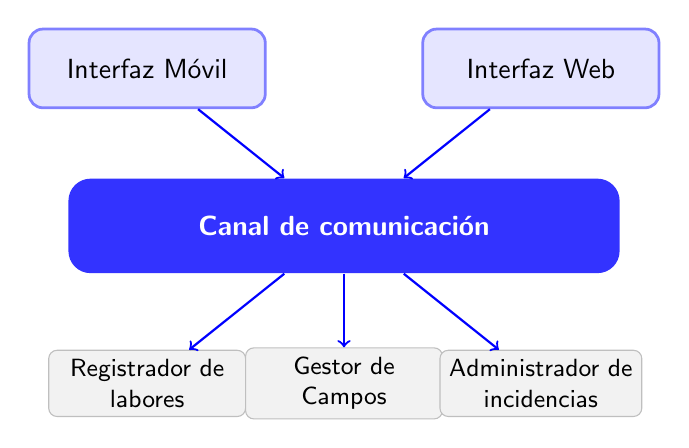
\begin{tikzpicture}[
    % Estilos máis simples pero modernos
        interface/.style={
            rectangle,
            rounded corners=5pt,
            fill=blue!10,
            draw=blue!50,
            line width=1pt,
            font=\sffamily,
            minimum width=3cm,
            minimum height=1cm,
            align=center
        },
        communication/.style={
            rectangle,
            rounded corners=8pt,
            fill=blue!80,
            text=white,
            font=\sffamily\bfseries,
            minimum width=7cm,
            minimum height=1.2cm,
            align=center
        },
        component/.style={
            rectangle,
            rounded corners=3pt,
            fill=gray!10,
            draw=gray!50,
            font=\sffamily\small,
            minimum width=2.5cm,
            minimum height=0.8cm,
            align=center
        }
    ]

        % Interfaces superiores
        \node[interface] (interfaz_movil) at (0, 3) {Interfaz Móvil};
        \node[interface] (interfaz_web) at (5, 3) {Interfaz Web};

        % Canal de comunicación
        \node[communication] (canal) at (2.5, 1) {Canal de comunicación};

        % Compoñentes inferiores
        \node[component] (registrador) at (0, -1) {Registrador de\\labores};
        \node[component] (gestor) at (2.5, -1) {Gestor de\\Campos};
        \node[component] (administrador) at (5, -1) {Administrador de\\incidencias};

        % Conexiones
        \draw[->, thick, blue] (interfaz_movil) -- (canal);
        \draw[->, thick, blue] (interfaz_web) -- (canal);
        \draw[->, thick, blue] (canal) -- (registrador);
        \draw[->, thick, blue] (canal) -- (gestor);
        \draw[->, thick, blue] (canal) -- (administrador);

    \end{tikzpicture}

    \begin{enumerate}
        \item Analiza detenidamente el diagrama y:
        \begin{enumerate}
            \item Asocia los componentes con los requisitos que cubren.
            \item Completa el diagrama con los componentes necesarios para cubrir todos los requisitos
            funcionales del Ejercicio 2.
        \end{enumerate}
        \item \textbf{0,4 puntos por cada requisito asociado.}
        \item \textbf{1 punto por completar el diagrama.}
    \end{enumerate}

\end{enunciado}

\begin{solucion}
    \begin{enumerate}
        \item Análisis del diagrama:
        \begin{enumerate}
            \item Asociaciones de componentes con requisitos:
            \begin{itemize}
                \item Interfaz web e interfaz móvil: Requisito 1.
                \item Gestor de campos: Requisitos 2 y 8.
                \item Registrador de labores: Requisito 3.
                \item Administrador de incidencias: Requisito 4.
            \end{itemize}

            \item Componentes necesarios para cubrir todos los requisitos funcionales:
            \begin{itemize}
                \item Gestor de producción: Conectado al canal de comunicación: Requisito 6.
            \end{itemize}
        \end{enumerate}
    \end{enumerate}
\end{solucion}